\chapter{Tendermint Consensus}
\label{ch:tendermint}

This chapter presents the Tendermint consensus algorithm 
and an associated blockchain for atomic broadcast.
The BFT consensus problem is described in detail, 
and a formal specification of Tendermint consensus is given in the $\pi$-calculus.
The Tendermint blockchain is informally proven to satisfy atomic broadcast.
We leave it to future work to capture the full blockchain protocol in 
a process calculus and to verify its properties.

\section{Tendermint Overview}

Tendermint is a secure state-machine replication algorithm in the blockchain paradigm.
It provides a form of BFT-ABC that is furthermore accountable - 
if safety is violated, it is always possible to verify who acted maliciously.

Tendermint begins with a set of \emph{validators}, identified by their public key,
where each validator is responsible for maintaining a full copy of the replicated state,
and for proposing new blocks (batches of transactions), and voting on them.
Each block is assigned an incrementing index, or \emph{height}, 
such that a valid blockchain has only one valid block at each height.
At each height, validators take turns proposing new blocks in \emph{rounds}, 
such that for any given round there is at most one valid proposer.
It may take multiple rounds to commit a block at a given height due to the asynchrony of the network,
and the network may halt altogether if more than one-third of the validators are offline or partitioned.
Validators engage in two phases of voting on a proposed block before it is committed, 
and follow a simple locking mechanism which prevents any coalition of up to 
one third malicious validators from compromising safety.

Note that the core round-based voting mechanism is the consensus algorithm, 
which is strung together into blocks to yield atomic broadcast.
Each block contains some metadata, known as its \emph{header}, 
which includes the hash of the block at the previous height, resulting in a hash chain.
The header also includes the block height, local time the block was proposed, 
and the Merkle root hash of transactions included in the block.

\section{Consensus}

The consensus algorithm can be roughly divided into the following, somewhat orthogonal, components:

\begin{itemize}

\item{Proposals: a new block must be proposed by the correct proposer at each round, and gossiped to the other validators. If a proposal is not received in sufficient time, the proposer should be skipped.}

\item{Votes: two phases of voting must occur to ensure optimal Byzantine fault tolerance. They are called \emph{pre-vote} and \emph{pre-commit}. $A$ set of pre-commits from more than two-thirds of the validators for the same block at the same round is a \emph{commit}.}

\item{Locks: Tendermint ensures that no two validators commit a different block at the same height, presuming less than one-third of the validators are malicious. This is achieved using a locking mechanism which determines how a validator may pre-vote or pre-commit depending on previous pre-votes and pre-commits at the same height. Note that this locking mechanism must be carefully designed so as to not compromise liveness.}

\end{itemize}

\begin{figure}[]
	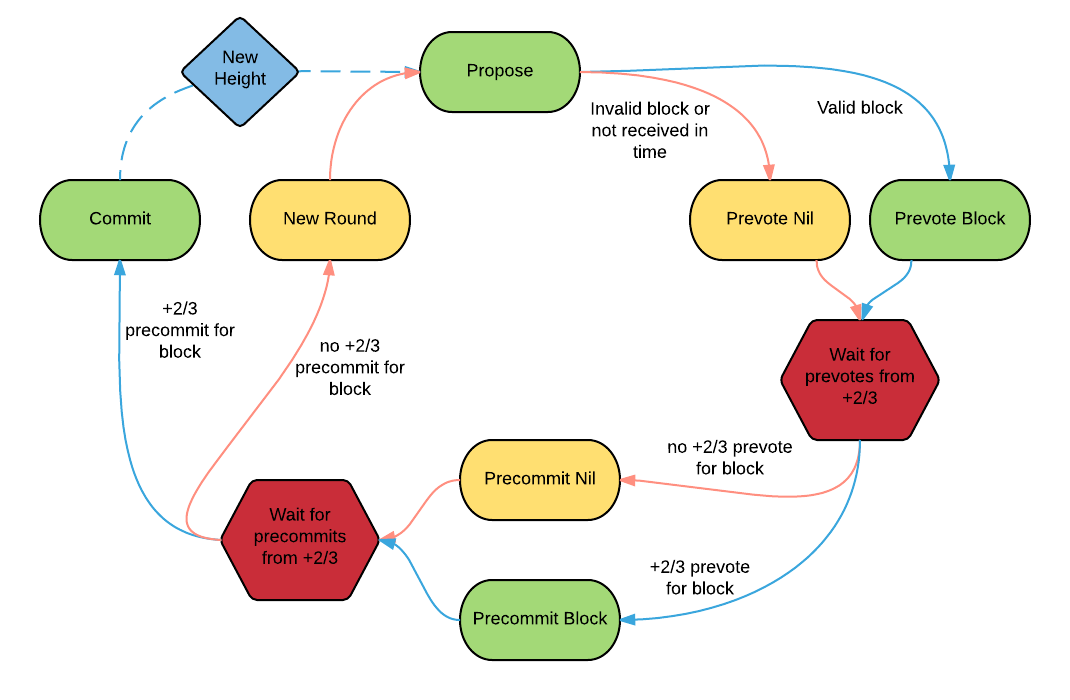
\includegraphics[width=\linewidth,height=\textheight,keepaspectratio]{figures/diagrams/consensus_logic.png}
    	\centering
	\caption[Overview of Tendermint consensus logic]{
After the proposal step, validators only make progress after hearing from two-thirds or more (+2/3) of other validators. The dotted arrow extends the consensus into atomic broadcast by moving to the next height.}
	\label{fig:consensus_logic}
\end{figure}

In order to provide tolerance to a single Byzantine fault, 
a Tendermint network must contain at minimum four validators.
Each validator must possess an asymmetric cryptographic key-pair for producing digital signatures.
Validators start from a common initial state, 
which contains the ordered list, $\mathcal{L}$, of validators.
Each validator is identified via their public key, and 
all proposals and votes must be signed by the respective private key.
This ensures that proposals and votes can always be verified by any observer.
It is helpful to assume that up to one-third of validators are malicious, 
co-operating in arbitrary ways to subvert system safety or liveness.

Consensus begins at round 0; the first proposer is the first validator in $\mathcal{L}$.
The outcome of a round is either a commit, or a decision to move to the next round.
With a new round comes the next proposer.
Using multiple rounds gives validators multiple opportunities 
to come to consensus in the event of network asynchrony or validator failures.

In contrast to algorithms which require a form of leader election, 
Tendermint has a new leader (the proposer) for each round.
Validators vote to skip to the next round in the same way they vote to accept the proposal,
lending the protocol a uniformity of mechanism that is absent 
from algorithms with an explicit leader-election program.

The beginning of each round has a weak dependence on synchrony as it utilizes local clocks to determine when to skip a proposer.
That is, if a validator does not receive a proposal within a locally measured \emph{TimeoutPropose} of entering a new round, it can vote to skip the proposer.
Inherent in this mechanism is the assumption that, at least eventually, the proposal will be delivered within \emph{TimeoutPropose}, which may itself increment with each round.
This assumption is discussed more fully in Chapter \ref{ch:related}.

After the proposal, rounds proceed in a fully asynchronous manner - a validator makes progress only after hearing from more than two-thirds of the other validators.
This relieves any sort of dependence on synchronized clocks or bounded network delays,
but implies that the network will halt if one-third or more of the nodes become unresponsive.
This circuit of weakly synchronous proposals, followed by asynchronous voting, 
is depicted in Figure \ref{fig:consensus_logic}.

To round-skip safely, a small number of \emph{locking} rules 
are introduced which force validators to justify their votes.
While we don't necessarily require them to broadcast their justifications in real time, 
we do expect them to keep the data,
such that it can be brought forth as evidence in the event that safety 
is compromised by sufficient Byzantine failures.
This accountability mechanism enables Tendermint to provide 
stronger guarantees in the face of such failure than eg.~PBFT,
which provides no guarantees if a third or more of the validators are Byzantine.

Validators communicate using a diverse set of messages for managing the blockchain, 
application state, peer network, and consensus.
The core consensus algorithm, however, consists of just two messages:

\begin{itemize}
\item{\emph{ProposalMsg}: a proposal for a block at a given height and round, signed by the proposer.}
\item{\emph{VoteMsg}: a signed vote for a proposal.}
\end{itemize}

In practice, we use additional messages to optimize the gossiping of block data and votes, as discussed in Chapter \ref{ch:subprotocols}.

\subsection{Proposals}

Each round begins with a proposal. 
The propser for the given round takes a batch of recently received transactions from its local cache (the Mempool, see Chapter \ref{ch:subprotocols}),
composes a block, and broadcasts a signed ProposalMsg containing the block.
If the proposer is Byzantine, it might broadcast different proposals to different validators.

Proposers are ordered via a simple, deterministic round robin, 
so only a single proposer is valid for a given round, 
and every validator knows the correct proposer. 
If a proposal is received for a lower round, or from an incorrect proposer, it is rejected.

Cycling of proposers is necessary for Byzantine tolerance. 
For instance, in Raft, if an elected leader is Byzantine and maintains strong network connections to other nodes,
it can completely compromise the system, destroying all safety and liveness guarantees.
Tendermint preserves safety via the voting and locking mechanisms, 
and maintains liveness by cycling proposers, so if one won't process any transactions, others can pick up.
Perhaps more interestingly, validators can vote through governance modules (see Chapter \ref{ch:governance}) to remove or replace Byzantine validators.

\subsection{Votes}

Once a complete proposal is received by a validator, 
it signs a pre-vote for that proposal and broadcasts it to the network.
If a validator does not receive a correct proposal within \emph{ProposalTimeout}, 
it prevotes for \emph{nil} instead.

In asynchronous environments with Byzantine validators, 
a single stage of voting, where each validator casts only one vote,
is not sufficient to ensure safety.
In essence, because validators can act fraudulently, 
and because there are no guarantees on message delivery time,
a rogue validator can co-ordinate some validators to commit a value
while others, having not seen the commit, 
go to a new round, within which they commit a different value.

A single round of voting allows validators to tell each other what they know about the proposal.	
But to tolerate Byzantine faults (which amounts, essentially to lies, fraud, deceipt, etc.), 
they must also tell each other what they know about what other validators have professed to know about the proposal.
In otherwords, a second stage ensures that enough validators witnessed the result of the first stage.

A pre-vote for a block is thus a vote to prepare the network to commit the block.
A pre-vote for nil is a vote to prepare the network to move to the next round.
In an ideal round with an online proposer, more than two-thirds of validators will pre-vote for the proposal.
A set of more than two-thirds of pre-votes for a single block at a given round is known as a \emph{polka}\footnote{The original term used was PoL, or PoLC, for Proof-of-Lock or Proof-of-Lock-Change. The term evolved to polka as it was realized the validators are doing the polka.}.
A set of more than two-thirds of pre-votes for nil is a \emph{nil-polka}

When a validator receives a polka (read: more than two-thirds pre-votes for a single block), 
it has received a signal that the network is prepared to commit the block,
and serves as justification for the validator to sign and broadcast a pre-commit vote for that block.
Sometimes, due to network asynchrony, a validator may not receive a polka, or there may not have been one. 
In that case, the validator is not justified in signing a pre-commit for that block, 
and must therefore sign and publish a pre-commit vote for nil.
That is, it is considered malicious behaviour to sign a pre-commit without justification from a polka.

A pre-commit is a vote to actually commit a block.
A pre-commit for nil is a vote to actually move to the next round.
If a validator receives more than two-thirds pre-commits for a single block, 
it commits that block, computes the resulting state,
and moves on to round 0 at the next height.
If a validator receives more than two-thirds pre-commits for nil,
it moves on to the next round.

\subsection{Locks}

Ensuring safety across rounds can be tricky, 
as circumstances must be avoided which would provide justification for two different blocks to be committed at two different rounds at the same height.
In Tendermint, this problem is solved via a \emph{locking} mechanism.
In essence, once a pre-commit is cast, a validator is \emph{locked} on the associated block, and must follow certain locking rules.
There are two rules of locking:

\begin{itemize}
\item{Prevote-the-Lock: a validator must pre-vote for the block they are locked on,
	and propose it if they are the proposer.	
	This prevents validators from pre-committing one block in one round, 
	and then contributing to a polka for a different block in the next round, 
	thereby compromising safety.}
\item{Unlock-on-Polka: a validator may only release a lock after seeing a polka at a round greater than that at which it locked.
	This allows validators to unlock if they pre-committed something the rest of the network doesn't want to commit,
	thereby protecting liveness, but does it in a way that does not compromise safety,
	by only allowing unlocking if there has been a polka in a round after that in which the validator became locked.}
\end{itemize}


For simplicity, a validator is considered to have locked on nil at round -1 at each height, 
so that Unlock-on-Polka implies that a validator cannot precommit at a new height until they see a polka.

These rules can be understood more intuitively by way of examples. 
Consider four validators, $A$, $B$, $C$, $D$, and suppose there is a proposal for $blockX$ at round $R$. 
Suppose there is a polka for $blockX$, 
but $A$ doesn't see it, and precommits nil, 
while the others precommit for $blockX$.
Now suppose the only one to see all precommits is D, 
while the others, say, don't see D's precommit (they only see their two precommits and A's precommit nil).
D will now commit the block, while the others go to round $R+1$.
Since any of the validators might be the new proposer, 
if they can propose and vote for any new block, say $blockY$, 
then they might commit it and compromise safety, since $D$ already committed $blockX$.
Note that there isn't even any Byzantine behaviour here, just asynchrony!

Locking solves the problem by forcing validators to stick with the block they pre-committed, 
since other validators might have committed based on those precommits (as $D$ did in this example).
In essence, once more than two-thirds precommit a block in a round, the network is locked on that block,
which is to say it must be impossible to produce a valid polka for a different block at a higher round.
This is direct motivation for Prevote-the-Lock.

Prevote-the-Lock is not sufficient, however. 
There must be a way to unlock, lest we sacrifice liveness.
Consider a round where $A$ and $B$ precommitted $blockX$ while $C$ and $D$ precommitted nil - a split vote.
They all move to the next round, and $blockY$ is proposed, which $C$ and $D$ prevote for.
Suppose $A$ is Byzantine, and prevotes for $blockY$ as well (despite being locked on $blockX$), resulting in a polka.
Suppose $B$ does not see the polka and precommits nil, while $A$ goes off-line and $C$ and $D$ precommit $blockY$. 
They move to the next round, but $B$ is still locked on $blockX$, while $C$ and $D$ are now locked on $blockY$, 
and since $A$ is offline, they can never get a polka. 
Hence, we've compromised liveness with less than a third (here, only one) Byzantine validators.

The obvious justification for unlocking is a polka. 
Once $B$ sees the polka for $blockY$ (which $C$ and $D$ used to jusitfy their precommits for $blockY$), 
it ought to be able to unlock, and hence precommit $blockY$.
This is the motivation for Unlock-on-Polka, 
which allows validators to unlock (and precommit a new block),
if they have seen a polka in a round greater than that in which they locked.

\subsection{Formal Specification}

Now that we have explained the protocol in detail, 
we provide a formal specification in the $\pi$-calculus.

%\begin{figure}[]
\begin{figure}[]
    	\centering
			
\begin{tabular}{l}
	\hline\\
	$Consensus := \prod_{i=1}^N  PR_i^{0,\emptyset,\emptyset,} $ \\\\

		\hline \\
		{$\!\begin{aligned}
		PR_i^{r,p,v} := 
			& \text{if } i=proposer(r) \text{ then } \\
				& \quad propose_i ! (prop) \| PV_i^{r,prop,v} \text{, where } prop = chooseProposal(p)\\
			& \text{ else if } p \neq \emptyset \text{ then}  \\
				& \quad PV_i^{r,p,v}  \\
			& \text{else} \\ 
				& \quad propose_{proposer(r)} ? (prop).PV_i^{r,prop,v} + susp_{proposer(r)}.PV_i^{r,\emptyset,v} \\
		\end{aligned}$} \\\\

		\hline \\
		$PV_i^{r,p,v}:= prevote_i ! (p) \| (\nu \> c) ( \prod_{j=1}^n prevote_j ? (w) . c!(prevote_j, w)  \| PV1_i^{r,p,v}(c))$ \\\\

		\hline \\
		{$\!\begin{aligned}
		PV1_i^{r,p,v}(c) := & \text{ if } max_{b}(|\left\{ w \in v_r^1 : w.block = b\right\}|) > \frac{2}{3} N \text{ then} \\
				& \quad PC_i^{r,b,v} \\
			& \text{else if }  | v_r^1 | > \frac{2}{3} N \text{ then} \\ 
				& \quad PC_i^{r,\emptyset,v} \\ 
			& \text{else} \\
				& \quad c?(pv, vote) . \text{ if } vote.round < r \text{ then} \\ 
						& \quad  \quad	pv?(w).c!(pv, w) \\ 
						& \quad  \text{else if } vote.round = r \text{ then} \\ 
						& \quad  \quad	PV1_i^{r,p,vote::v}(c) \\
						& \quad  \text{else } \\
						& \quad  \quad PR_i^{vote.round, p, vote::v} \\
		\end{aligned}$} \\\\
		\hline\\

\end{tabular}

	\caption[Formal specification of Tendermint consensus in the $\pi$-calculus, part I]{Formal specification of Tendermint consensus in the $\pi$-calculus, part I.
$chooseProposal(p)$ must return $p$ if it is not $\emptyset$, and otherwise should gather transactions from the mempool as described in Chapter \ref{cite:subprotocols}. 
After receiving a proposal or timing out, validators move onto prevote,
where they broadcast their prevote and wait to receive prevotes from the others.
If a vote is received for a later round, we skip ahead to that round.
 }
	\label{fig:tendermint_pi1}
\end{figure}

\begin{figure}[]
    	\centering
			
\begin{tabular}{l}
		\hline \\
		$PC_i^{r,p,v}:= precommit_i ! (p) \| (\nu \> c) ( \prod_{j=1}^n precommit_j ? (w) . c!(w)  \| PC1_i^{r,p,v}(c))$ \\\\

		\hline \\
		{$\!\begin{aligned}
		PC1_i^{r,p,v}(c) := 
			& \text{ if } max_{b}(|\left\{ w \in v_r^2 : w.block = b\right\}|) > \frac{2}{3} N \text{ then} \\
				& \quad d_i!(b) \\
			& \text{else if }  | v_r^2 | > \frac{2}{3} N \text{ then} \\ 
				& \quad PR_i^{r+1,\emptyset,v} \\ 
			& \text{else} \\
				& \quad c?(pc, vote) .\text{ if } vote.round < r \text{ then} \\ 
						& \quad  \quad	pc?(w).c!(pc, w) \\ 
						& \quad  \text{else if } vote.round = r \text{ then} \\ 

						& \quad  \quad	PC1_i^{r,p,vote::v}(c) \\
						& \quad  \text{else } \\
						& \quad  \quad PR_i^{vote.round, p, vote::v} \\
		\end{aligned}$} \\\\
		\hline\\

\end{tabular}

	\caption[Formal specification of Tendermint consensus in the $\pi$-calculus, part II]{Formal specification of Tendermint consensus in the $\pi$-calculus, part II.
Validators broadcast their precommit and wait to receive precommits from the others.
If a vote is received for a later round, we skip ahead to that round.
When more than two-thirds pre-commit for block $b$, we fire $b$ on channel $d_i$, signalling the commit,
and terminating the protocol.
}
	\label{fig:tendermint_pi}
\end{figure}


Let $Consensus := \prod_{i=1}^N Y_i $ represent a consensus protocol
over a set of $N$ validators, each executing one of a mutually exclusive set of processes, $Y_i$.
Internal state $s = \{r, p, v \}$ consists of a strictly increasing round, $r$,
a proposal $p$, containing the proposed block for this round;
and a set of votes, $v$, containing all votes at all rounds;
We denote by $v_r^1$ and $v_r^2$ the set of prevotes and precommits, respectively, at round $r$.
We define $proposer(r) = r \mod N$ to be the index of the proposer at round $r$.
We represent a peer at a particular point in the protocol as $Y_i^{r, p, v}$.
Processes $Y_i$ range over $PR_i$, $PV_i$, $PC_i$, 
respectively abbreviating 
\emph{propose}, \emph{prevote}, \emph{precommit}.
We introduce additional sub-functions for $PV$ and $PC$ to capture the recursion,
denoted $PV1$, $PV2$, etc.

Peers are connected using broadcast channels for each message type,
namely $propose_i$, $prevote_i$, and $precommit_i$,
as well as a channel for deciding on, or committing, a value, $d_i$.
Via an abuse of notation, a single send on a broadcast channel $xxx_i$ can be received by each process along
$xxx_i$.

We use only two message types: proposals and votes. 
Each contains a round number, block (hash), and signature, 
denoted $msg.round$, $msg.block$, $msg.sig$.
Note we can absorb the signature into the broadcast channel itself,
but we need it for use as evidence in the event of Byzantine behaviour.

The specification is given in two parts, in Figures \ref{fig:tendermint_pi1} and \ref{fig:tendermint_pi2}.

\section{Blockchain}

Tendermint operates on batches, or blocks, of transactions at a time.
Continuity is maintained from one block to the next by explicitly linking each block to the one before it 
via it's cryptographic hash, forming a blockchain. 
The blockchain contains both the ordered transaction log and evidence that the block was committed 
by the validators.

\subsection{Why Blocks?}
Consensus algorithms typically commit transactions one at a time by design, 
and implement batching after the fact.
As mentioned in Chapter \ref{ch:background}, 
tackling the problem from the perspective of batched atomic broadcast
results in two primary optimizations, which give us more throughput and fault-tolerance:

\begin{itemize}
\item{Bandwidth optimization: since every commit requires two rounds of communication across all validators, 
	batching transactions in blocks amortizes the cost of a commit over all the transactions in the block.}
\item{Integrity optimization: the hash chain of blocks forms an immutable data structure, much like a Git repository, enabling authenticity checks for sub-states at any point in the history.}
\end{itemize}

Blocks induce another effect as well, which is more subtle but potentially important. 
They increase the minimum latency of a transaction to that of the whole block, 
which for Tendermint is on the order of hundreds of milliseconds to seconds.
Traditional serializable database systems provide commit latencies on the 
order of milliseconds to tens of milliseconds.
They are able to do this because they are not Byzantine Fault Tolerant, 
requiring only one round of communication (instead of two)
and responses from over half of the replicas (instead of two-thirds).
However, unlike the fast commit times interrupted by leader elections in other algorithms,
Tendermint provides a more regular pulse that is more responsive to the overall health of the network, 
in terms of node failures and asynchrony.

What role such pulses might play in the coherence of 
communicating autonomous systems on the internet is yet to be determined,
though purposefully induced latency has shown promise in the financial markets \cite{ryan2015beyond}.

\subsection{Block Structure}

The purpose of blocks is to contain a batch of transactions, and to link to the previous block.
The link comes in two forms: the previous block hash,
and the set of pre-commits which caused the previous block to be committed, also known as the $LastCommit$.
Thus a block is composed of three parts: the block header, the list of transactions, and the $LastCommit$.

\section{Safety}

Here we sketch a brief proof that Tendermint satisfies atomic broadcast,
which is defined as satisfying:

\begin{itemize}
\item validity - if a correct process broadcasts $m$, it eventually delivers $m$
\item agreement - if a correct process delivers $m$, all correct processes eventually deliver $m$
\item integrity - $m$ is only delivered once, and only if broadcast by its sender
\item total order - if correct processes $p$ and $q$ deliver $m$ and $m'$, then $p$ delivers $m$ before $m'$ iff $q$ delivers $m$ before $m'$
\end{itemize}

Note that if we take $m$ to be a block,
Tendermint does not satisfy validity,
since there is no guarantee that a proposed block is eventually committed, 
as validators may move to a new round and commit a different block.
If we take $m$ to be a batch of transactions in a block, 
then we can satisfy validity by having validators re-propose the same batch until it is committed.
However, to satisfy the first half of integrity 
we must introduce an additional rule that forbids a correct validator from 
proposing a block or pre-committing for a block containing a 
batch of transactions that has already been committed.
Fortunately, batches can be indexed by their merkle root,
and a lookup performed before proposals and pre-commits.

Alternatively, if we take message $m$ to be a transaction, 
then we can satisfy validity by asserting a \emph{persistence}
property on the mempool, namely, that a transaction persists in the mempool 
until it is committed.
However, to satisfy the first half of integrity we must 
rely on the application state to enforce some ruleset over 
transactions such that a given transaction is only valid once. 
This can be done, for instance, using sequence numbers on accounts,
as is done in ethereum, 
or by keeping a list of unused resources, each of which can only be used once,
as is done in Bitcoin.
Since there are multiple approaches,
Tendermint does not in itself ensure that a message is only delivered once,
but allows the application developer to specify.
Note that the second half of integrity is trivially satisfied,
since only transactions in blocks proposed by a correct proposer can be committed.

To show that Tendermint satisfies the remaining properties,
we introduce a new property, \emph{state machine safety},
and show that a protocol satisfing state machine safety satisfies
agreement and total order.
State machine safety states that if a correct validator commits a block at some height $H$,
no other correct valdiator will ever commit a different block at $H$.
Given that all messages are eventually received, 
this immediately implies agreement, since if a correct validator commits a block $B$ at height $H$ 
containing a transaction $m$, all other correct validators will be unable to commit any other block,
and hence must eventually commit $B$, thereby delivering $m$.

Now, it remains to show that state machine safety satisfies total order,
and that Tendermint satisfies state machine safety.
To see the former, consider two messages $m$ and $m'$ delivered by validators $p$ and $q$.
State machine safety ensures that $p$ delivers $m$ at height $H_m$ if and only if
$q$ delivers $m$ at height $H_m$, and that $p$ delivers $m'$ at height $H_{m'}$ 
if and only if $q$ delivers $m'$ at height $H_{m'}$. 
Without loss of generality, and since height is strictly increasing, let $H_m < H_{m'}$.
Then we have that $p$ delivers $m$ before $m'$ if and only if $q$ delivers $m$ before $m'$,
which is exactly the statement of total order.

Finally, to show Tendermint satisfies state machine safety when less than a third of 
validators are Byzantine, we proceed by way of contradiction.
Suppose Tendermint does not satisfy state machine safety, 
allowing more than one block to be committed at the same height.
Then we show that at least one-third of validators must be Byzantine for that to happen,
contradicting our assumption.

Consider a correct validator having committed block $B$ at height $H$ and round $R$.
To commit a block means the validator witnessed pre-commits 
for block $B$ in round $R$ from more than two-thirds of validators.
Suppose another block $C$ is committed at height $H$. 
We have two options: either it was committed in round $R$, or round $S > R$.

If it was committed in round $R$, then more than two-thirds of validators
must have pre-committed for it in round $R$, which means that at least a third of validators 
pre-committed for both blocks $B$ and $C$ in round $R$, which is clearly Byzantine.
Suppose block $C$ was instead committed in round $S > R$.
Since more than two-thirds pre-committed for $B$, they are locked on $B$ in round $S$,
and thus must pre-vote for $B$. To pre-commit for block $C$, they must 
witness a polka for $C$, which requires more than two-thirds to pre-vote for $C$.
However, since more than two-thirds are locked on and required to pre-vote for $B$,
a polka for $C$ would require at least one third of validators to violate Prevote-the-Lock,
which is clearly Byzantine.
Thus, to violate state machine safety, at least one third of validators must be Byzantine.
Therefore, Tendermint satisfies state machine safety when less than a third of validators are Byzantine.

Given the above, then, Tendermint satisfies atomic broadcast.

In future work, we aim to provide a more formal proof of Tendermint's safety property.

%
%- Proposer Safety condition implied by protocol
%- Validator Append Only condition implied by the protocol
%- Proposer Completeness guaranteed by the merkle hash chain
%
%Need to show Block Matching, State Machine Safety, and Deterministic Accountability.
%Locking rules give us lemmas about polkas.
%


\section{Accountability}

An accountable BFT algorithm is one that can identify all Byzantine validators 
when there is a violation of safety. 
Traditional BFT algorithms do not have this property,
and provide no guarantees in the event safety is compromised.
Of course, accountability can only apply when between one-third and two-thirds of
validators are Byzantine.
If more than two-thirds are Byzantine, they can completely dominate the protocol,
and we have no guarantee that a correct validator will receive any evidence of their misdeeds.

Futhermore, accountability can be at best eventual in asynchronous networks - 
following a violation of safety, the delayed delivery of critical messages
may make it impossible to determine which validators were Byzantine until some time after
the safety violation is detected. 
In fact, if correct processes can receive evidence of Byzantine behaviour, 
but fail irreversibly before they are able to gossip it, 
there may be cases where accountability is permanently compromised,
though in practice such situations should be surmountable
with advanced backup solutions.

By enumerating the possible ways in which a violation of safety can occur,
and showing that in each case, the Byzantine validators are identifiable,
a protocol can be shown to be accountable.
Tendermint's simplicity affords it a much simpler analysis than protocols 
which have to manage leadership elections.

There are only two ways for a violation of safety to occur in Tendermint,
and both are accountable.
In the first, a Byzantine proposer makes two conflicting proposals within a round,
and Byzantine validators vote for both of them.
In the second, Byzantine validators violate locking rules after some validators have already committed,
causing other validators to commit a different block in a later round.
Note that it is not possible to cause a violation of safety with two-thirds or fewer
Byzantine validators using only violations of Unlock-on-Polka - 
more than a third must violate Prevote-the-Lock for their to be a polka justifying a commit 
for the remaining honest nodes.

In the case of conflicting proposals and conflicting votes,
it is trivial to detect the conflict by receiving both messages,
and to identify culprits via their signatures.

In the case of violating locking rules, following a violation of safety,
correct validators must broadcast all votes they have seen at that height, 
so that the evidence can be stitched together.
The correct validators, which number something under two-thirds, 
were collectively privy to all votes which caused the two blocks to be committed.
Within those votes, if there are not a third or more validators signing conflicting votes,
then there are a third or more violating Prevote-the-Lock.

If a pre-vote or a pre-commit influenced a commit, it must have been seen by a correct validator.
Thus, by collecting all votes, violations of Prevote-the-Lock can be detected
by matching each pre-vote to the most recent pre-commit by the same validator, unless there isn't one.

Similarly, violations of Unlock-on-Polka can be detected by matching each pre-commit
to the polka that justifies it. 
Note that this means a Byzantine validator can pre-commit before seeing a polka,
and escape accountability if the appropriate polka eventually occurs.
However, such cases cannot actually contribute to violations of safety 
if the polka is happening anyways.

The current design provides accountability following a post-crisis broadcast protocol,
but it could be improved to allow accountability in real time. 
That is, a commit could be changed to include not just the precommits, but all votes 
justifying the precommits, going all the way back to the beginning of the height.
That way, if safety is violated, the unjustified votes can be detected immediately.

\section{Faults and Availability}

As a BFT consensus algorithm, Tendermint can tolerate Byzantine failure in up to 
(but not including) one-third of validators.
This means nodes can crash, send different and contradictory messages to different peers, 
refuse to relay messages, or otherwise behave arbitrarily,
without compromising safety or liveness (with the usual FLP caveat for liveness).

There are two places in the protocol where we can make optimizations 
for asynchrony by utilizing timeouts based on local clocks:
after receiving two-thirds or more pre-votes, but not for a single block or nil, 
and after receiving two-thirds or more pre-commits, 
but not for a single block or nil.
In each case, we can sleep for some amount of time to give slower or delayed votes a chance to be received,
thereby reducing the likelihood of going to a new round without committing a block.
Clocks do not need to be synced across validators, 
as they are reset each time a validator observes votes from two-thirds or more others.

If a third or more of validators crash, the network halts, 
as no validator is able to make progress without hearing from more than two-thirds of the validator set.
The network remains available for reads, but no new commits can be made.
As soon as validators come back on-line, they can carry on from where they left in a round. 
The consensus state-machine should employ a write-ahead log,
such that a recovered validator can quickly return to the step it was in when it crashed,
ensuring it doesn't accidentally violate a rule.

If a third or more of validators are Byzantine, they can compromise safety a number of ways, 
for instance, by proposing two blocks for the same round, and voting both of them through to commit, 
or by pre-committing on two different blocks at the same height but in 
different rounds by violating the rules on locking.
In each case, there is clear, identifiable evidence that certain validators misbehaved. 
In the first instance, they signed two proposals at the same round, a clear violation of the rules.
In the second, they may have pre-voted for a different block in round $R$ than they locked on in $R-1$, 
a violation of the Prevote-the-Lock rule.

When using economic and governance components to incentivize 
and manage the consensus (Chapter  \ref{ch:governance})
these additional accountability guarantees become critical.

\section{Conclusion}

Tendermint is a weakly synchronous, Byzantine fault tolerant, state machine replication protocol,
with optimal Byzantine fault tolerance and additional accountability guarantees in the event
the BFT assumptions are violated. 
The protocol uses a round-robin approach for proposers, and uses the same mechanism to skip a proposer as to commit a proposed block.
Safety is maintained across rounds via a simple locking mechanism.

The presentation of the protocol in this chapter left out many important details, 
such as the efficient gossiping of blocks, buffering transactions, changes to the validator set, 
and the interface with application logic. These important topics are taken up in subsequent chapters.


